
\chapter{Aplicaciones del análisis de Fourier}
\section{Desarrollo de Fourier}
\textbf{Idea del análisis de Fourier:} "toda" señal se puede descomponer en "tonos puros" (armónicos) de frecuencia fija (típicamente $\sin(\alpha n x)$ , $\cos(\alpha n x)$  $ n \in \ent$).

%Dibujo con caption ($\frac{1}{4} - \frac{2}{\pi^2} \sum_{n impares} \frac{1}{n^2} \cos(2\pi n x)$)

\begin{example}
Sea la función $f(t)=t$ con $t\in[0,1)$ que se ha extendido periódicamente con período $T=1$.

\begin{center}
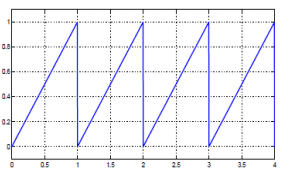
\includegraphics[width=\linewidth]{img/id_period.png}
\end{center}

Su desarrollo de fourier (que veremos más adelante cómo se calcula) queda de la forma:
\[SF(f(t))=\frac{1}{2}-\frac{1}{π}\sum_{n=1}^{\infty}\frac{1}{n}\sin(2πnt)\]

Cuántos más elementos del sumatorio tomemos más precisa será la proximación:

\begin{center}
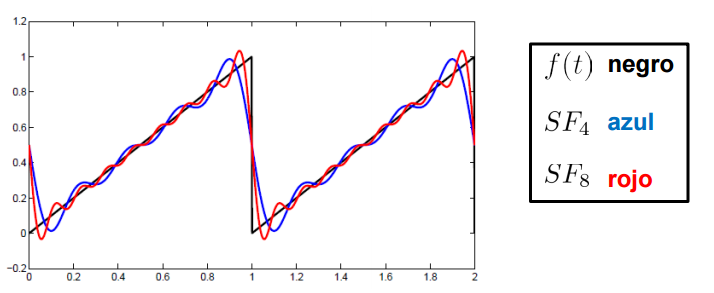
\includegraphics[width=\linewidth]{img/id_period_fourier.png}
\end{center}

	%Cogemos $x=0$:
	%$$0 = \frac{1}{4} - \frac{2}{\pi^2} \sum_{\text{n impares}} \frac{1}{n^2}$$
	%$$1 + \frac{1}{3^2} + \frac{1}{5^2} + \ldots = \frac{\pi^2}{8}$$
\end{example}

\subsection{Aplicaciones}
\begin{itemize}
	\item Muchas aplicaciones de ingeniería están basadas en estas ideas. (JPEG, MP3, MPEG, telecomunicaciones)

	Hay tonos puros (frecuencias) que se eliminan o modifican porque no tienen mucha influencia o son ruido.

	Menos frecuencia $\rightarrow$ Menos información $\rightarrow$ Compresión (pérdidas)

	En ingeniería una aplicación muy común es utilizar esto como filtro, en el caso del MP3 se eliminan las frecuencias que no oímos.

	\item En matemáticas y física: Hay problemas difíciles para funciones generales y fáciles para "tonos puros" (senos y cosenos).

		\textbf{Interpretación de Copenhague}: Las partículas tienen funciones de ondas y en los experimentos sólo se detectan los tonos puros que componen estas funciones con una probabilidad que depende de su amplitud.

	%Vamos a ver aplicaciones de esto:

	%\textbf{\textit{Pasar de analógico a digital}}

	%Vamos a hacer análisis de Fourier discreto con ondas digitalizadas.

%	\begin{example}
%		Vamos a estudiar la función $\sin\left(\frac{2\pi}{T}\cdot x\right)$
%
%		Dibujo
%
%		que es un caso particular de $\sin\left(\frac{2\pi}{T}\cdot k x\right)$ (oscila k veces en [0,T]).

%		Dibujo

%		Si digitalizamos la función, hacemos que x solo tenga valores discretos: $\sin\left(\frac{2\pi}{T}\cdot n\right)$

%		Dibujo

%		LLamamos $f(n)$ a la función discretizada, $n \in \ent$ ; Con N periódica $f(n + N) = f(n)$

%		Matemáticamente pensamos $f(n)$ como :
%		$$f : \ent/N\ent \rightarrow \mathbb{C} $$
%	\end{example}
	\obs En general consideramos que el recorrido de $f$ es $\mathbb{C}$ porque $e^{ix} = \cos x + i\sin x$ permite escribir senos y cosenos al mismo tiempo.

	$$\cos x = \frac{e^{ix} + e^{-ix}}{2}$$
	$$\sin x = \frac{e^{ix} - e^{-ix}}{2i}$$

\end{itemize}

\begin{theorem}[Análisis de Fourier en $\ent/N\ent$]

	Cualquier $f : \ent/N\ent \rightarrow \mathbb{C}$ se puede escribir como :
	$$f(n) = \frac{1}{N}\sum_{m\in \ent/N\ent}\widehat{f}(m)\cdot e\left(\frac{nm}{N}\right)$$
	donde $e(x) = e^{2\pi ix}$

	$\widehat{f}(n)$ es la \textbf{transformada de Fourier discreta}
	$$\widehat{f}(n) = \sum_{m\in \ent/N\ent}\widehat{f}(m)\cdot e\left(\frac{-nm}{N}\right)$$

\end{theorem}
\obs Hay un algoritmo eficiente para calcular los $\widehat{f}(m)$ llamado Transformada Rápida de Fourier (en inglés Fast Fourier Transform, TTF)

\begin{proof}
	Definimos la función $\delta : \ent/N\ent \rightarrow \mathbb{C}$ como :
	$$\delta (n) = \begin{cases}
	1 \text{ si } n=0\\
	0 \text{ si } n\neq 0 \\
	\end{cases}$$
	Y decimos que también se puede escribir como:
	$$\delta (n) = \frac{1}{N} \sum_{m = 0}^{N-1} e\left(-\frac{nm}{N}\right)$$
	Donde
	\[e\left(\frac{nm}{N}\right) = e^{\frac{2\pi inm}{N}}\]

	Es claro que $\delta(0) = 1$, pero aún tenemos que ver que $n\neq 0 \implies \delta (n) = 0$

	Podemos ver δ como el producto de $\frac{1}{N}$ por la suma de los términos de una progresión geométrica tal que:
	\[\begin{cases}
	a_1 = e(n0/N)=e(0)=1\\
	a_{n+1} = e(-nN/N)=e(n)\\
	\text{razón } = e^{-\frac{n}{N}}
	\end{cases}\]

	Basándonos en la fórmula conocida para la suma de los términos de una progresión geométrica tenemos:
	$$\delta (n) =\frac{e(n) - e(0)}{e^{n/N} - 1} = 0$$

	Otra forma de pensarlo es como vectores. $\delta(n)$ se puede ver como la suma de todas las raíces de la unidad. Si lo vemos como las raíces de la unidad podemos entender cada raíz como un vector que representa una fuerza aplicada con el origen, con lo que vemos fácilmente que todas esas fuerzas se anulan lo que encaja con la idea de que la suma de las raíces de la unidad es 0.

	%(dibujo explicativo para N=4)

	Una vez que tenemos esto, vemos que la $f(n)$ del teorema se puede escribir como:
	$$f(n) = \sum_{k\in \ent/N\ent} f(k) \cdot \delta(n-k)$$
	puesto que fijado un $n$ todos los sumanos serán 0 excepto aquel en que $n=k$ con lo que obtenemos la igualdad trivial $f(n)=f(n)$

	Sustituyendo:
	$$f(n) =\frac{1}{N} \sum_{k\in \ent/N\ent} f(k)  \sum_{m \in \ent/N\ent} e\left(\frac{(n-k)m}{N}\right) =  \frac{1}{N} \sum_{k\in \ent/N\ent} f(k)  \sum_{m \in \ent/N\ent} e\left(\frac{nm}{N}\right) \cdot e\left(- \frac{km}{N}\right)$$

	Y como por definición:
	$$\widehat{f}(m) = \sum_{k\in \ent/N\ent} f(k) \cdot e\left(- \frac{km}{N}\right)$$

	Pues ya está probado el teorema.
\end{proof}
\begin{example}
	Vamos a hacer un ejemplo con $N=3$. Supongamos que tenemos los siguientes datos de una función, que sabemos que es periódica a intervalos de longitud 2 empezando en el origen:
	$$f(n) = \begin{cases}
	7 \text{ si } n= 0\\
	2 \text{ si } n = 1 , 2
	\end{cases}$$

	Entonces aplicando la fórmula del teorema nos queda:
	$$\widehat{f}(0) = f(0)\cdot e(0) + f(1)\cdot e(0) + f(2) \cdot e(0) =  11$$
	$$\widehat{f}(1) = f(0)\cdot e(0) + f(1)\cdot e\left(-\frac{1}{3}\right) + f(2)\cdot e\left(-\frac{2}{3}\right) = 7 + 2\cdot\left(-\frac{1}{2} -i\frac{\sqrt{3}}{2}\right) + 2\cdot \left(-\frac{1}{2} + \frac{i\sqrt{3}}{2}\right) = 5$$
	$$\widehat{f}(2) = f(0)\cdot e(0) + f(1)\cdot e\left(- \frac{2}{3}\right) + f(2) \cdot e\left(-\frac{4}{3}\right) = 7 + 2\cdot\left(-\frac{1}{2} -i\frac{\sqrt{3}}{2}\right) + 2\cdot \left(-\frac{1}{2} + \frac{i\sqrt{3}}{2}\right) = 5$$
	Como
	$$f(n) = \frac{1}{N} \sum_{m\in \ent/ N\ent} \widehat{f}(m) \cdot e\left(\frac{nm}{N}\right)$$
	Sustituyendo con los resultados de antes nos queda que:
	$$f(n) = \frac{11}{3}\cdot e\left(0 \cdot \frac{n}{3}\right) + \frac{5}{3}\cdot e\left(1 \cdot \frac{n}{3}\right) + \frac{5}{3} \cdot e\left(2 \cdot \frac{n}{3}\right)$$

	Y efectivamante, si comparamos resultados nos queda :
	$$n = 0 \rightarrow 7 = \frac{11}{3} + \frac{5}{3} + \frac{5}{3}$$
	$$n = 1 \rightarrow 2 = \frac{11}{3} + \frac{5}{3} \cdot \left(- \frac{1}{2} + \frac{i \sqrt{3}}{2}\right) + \frac{5}{3} \cdot \left(- \frac{1}{2} -\frac{i \sqrt{3}}{2}\right)$$
\end{example}

Este teorema se puede utilizar para \textbf{transformar funciones discretas(con N grande) a funciones continuas}.

\begin{center}
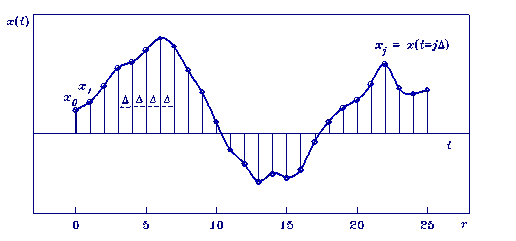
\includegraphics[width=\linewidth]{img/fourier_discreta_a_continua.png}
\end{center}

Tenemos f(n) discreta, llamamos $F\left(\frac{n}{N}\right) = f(n)$ a la función continua que queremos construir.


Haciendo el desarrollo de Fourier de f nos queda que:
$$f(n) = \sum \frac{\widehat{f}(m)}{N} \cdot e\left(\frac{nm}{N}\right)$$

Llamamos $x = \frac{n}{N}$ y $a_m= \frac{\widehat{f}(m)}{N}$ y nos queda que :
$$F(x) = \sum_{n\in \ent } a_m \cdot e(mx)$$

Para calcular $F(x)$ necesitamos calcular primero el $a_m$. Para ello hacemos el límite de $\frac{\widehat{f}(m)}{N}$

Entonces tenemos que:
$$\frac{\widehat{f}(m)}{N} = \frac{1}{N} \sum_{k \in \ent/N\ent} f(k) \cdot e\left(-m \frac{k}{N}\right) \text{ con } \begin{cases}
	m \text{ fijo}\\
	N \text{ muy grande}\\
	f(k) = F\left(\frac{k}{N}\right)\\
\end{cases}$$

Como $ k = 0 , \ldots , N-1 \implies 0\leq \frac{k}{N} < 1$ podemos interpretar el sumatorio como suma de Riemann de modo que:

$$\frac{\widehat{f}(m)}{N} = \int_{0}^{1} F(x) \cdot e(-mx) dx$$

Finalmente obtenemos:
$$F(x) = \sum_{m= -\infty}^{\infty} \widehat{F}(n) \cdot e(nx) \text{ siendo } \widehat{F}(n) = \int_{0}^{1} F(x) \cdot e(-nx) dx$$

\obs La no acotación de $\real$ limita la validez de esta fórmula para funciones $F$  buenas (por ejemplo $C^2$).



%%% CLASES POR  REVISAR



$ f: \mathbb{R} \rightarrow \mathbb{C} $ 1-periódica

$f(x) = \sum\limits_{n=-\infty}^{\infty} \hat{f}(n) e(nx) \;\;\;\;\;\; \hat{f}(n) = \int\limits_{0}^{L} f(x) e (-nx) dx \;\;\;\; e(x) = e^{2 \pi i x}$

$f(x) \equiv $ Desarrollo de Fourier de f \;\;\;\; $\hat{f}(n) =$ coeficientes de Fourier de f.

La igualdad $f(x) = \sum^{\infty}_{n=-\infty}$ es cierta para $f$ periódica $\in C^{2}$ y la convergencia es uniforme (Tma. de Carlesson-Hunt $\Rightarrow$ la igualdad es cierta en casi todo punto con tal de que $f \in L^{P} [0,1] p > 1$)

¿Se puede analizar en senos y cosenos una función no periódica? Sí, pero hay que tomar los de frecuencias no enteras.

$g \equiv $ función 1-periódica $ \Rightarrow f(x) = g(\frac{x}{T})$ es T-periódica.

$$ g(x) = \sum^{\infty}_{n=-\infty} \hat{g}(n) e(nx) \;\;\; \hat{g}(n) = \int\limits^{1}_{0} = \int\limits^{1/2}_{-1/2} g(x) e(-nx) dx $$

$x |\rightarrow \frac{x}{T} $

$$f(x) = \sum_{n = -\infty}^{\infty} \hat{g}(n) e(\frac{n}{T}x) \;\;\; \hat{g}(n) = \frac{1}{T} \int\limits^{T/2}_{-T/2} f(y) e(-\frac{n}{T}y) dy$$

$$f(x) = \frac{1}{T} \sum_{n = -\infty}^{\infty} \left(  \int\limits^{T/2}_{-T/2} f(y) e(-\frac{n}{T}y) dy \right) e (\frac{n}{T}x)$$

$T \rightarrow \infty$ Escribiendo $\frac{n}{T} = \psi$

$$ f(x) =^{?} \int\limits^{\infty}_{-\infty} \text{ otra integral } e(\psi x) d\psi $$

Esto sugiere que para $f: \mathbb{R} \rightarrow \mathbb{C}$

$$f(x) = \int\limits^{\infty}_{-\infty} \hat{f}(\psi) e (x \psi) d \psi \text{ donde } \hat{f}(\psi) = \int\limits^{\infty}_{-\infty} f(y) e(-\psi y)dy$$

$\hat{f}$ se conoce como la transformada de Fourier (y se inventó antes que la discreta). Y $f(x)$ es la Fórmula de inversión.

La igualdad $f(x) = \int\limits^{\infty}_{-\infty} $... es cierta para $f$ que decaiga rápido con cierta regularidad.

%% Hasta aquí no hay quien cojones lea nada
\newpage
\textbf{RESUMEN:}

\begin{itemize}

\item Si tenemos una función $f$ : $\mathbb{Z}_{n} = \mathbb{Z} / n \mathbb{Z} \rightarrow \mathbb{C}$ su desarrollo discreto de fourier nos dice:

$$ f(n) = \frac{1}{n} \sum_{m \in \mathbb{Z}_{n}} \hat{f}(m) e \left( \frac{mn}{N} \right) $$

$$ \hat{f}(n) = \sum_{m \in \mathbb{Z}_{n}} f(m) e \left( \frac{-mn}{N} \right)$$

\item Si tenemos una función $\appl{f}{\mathbb{T}}{\cplex}$, es decir, una función 1-periódica el desarrollo de fourier queda:

$$ f(x) = \sum^{\infty}_{n = -\infty} \hat{f} (n) e (nx) $$

$$ \hat{f} (n) = \int\limits_{0}^{1} f(x) e (-nx) dx $$

\item Para f: $\mathbb{R} \rightarrow \mathbb{C}$

$$ f(x) = \int\limits^{\infty}_{-\infty} \hat{f}(\psi) e(x \psi) d\psi $$

$$ \hat{f}(\psi) = \int^{\infty}_{-\infty} f(x) e(-\psi x)dx$$

\end{itemize}

\obs En los dos últimos casos serán necesarias ciertas condiciones de regularidad sobre la función $f$

\begin{example}

	Hallar el desarrollo de Fourier de la función 1-periódica que en $[-1/2, 1/2]$ vale
	\[f(x)=e^{2\pi x} + e^{-2\pi x } = 2 \cosh (2 \pi x)\]

	Para empezar calculamos la fórmula general de los coeficientes de la serie de fourier:
	$$\hat{f}(n) = \int ^{1/2}_{-1/2} \left( e^{2 \pi x} + e ^{-2 \pi x} \right) e ^{-2 \pi i n x} = \frac{1}{2 \pi} (e^{\pi} - e^{-\pi}) (-1)^{n} \left( \frac{1}{1-in} + \frac{1}{1 + in} \right) =$$

	Y ahora calculamos la serie propiamente dicha:
	$$ = \frac{e^{\pi} - e^{-\pi}}{\pi} (-1)^{n} \frac{1}{1 + n^2}$$

	$$ f(x) = e ^{2 \pi x} + e^{-2 \pi x} = \frac{e^{pi} - e^{-\pi}}{\pi} \sum_{n = -\infty}^{\infty} \frac{(-1)^n}{1 + n^2} e(nx) $$

\end{example}


\begin{example}{Otro ejemplo}

Expresar $e^{-|x|}$ como una integral usando la fórmula de inversión.


Recordemos la fórmula de inversión:

$$ f(x) = \int\limits^{\infty}_{-\infty} \hat{f}(\psi) e(x\psi) d\psi \rightarrow \hat{f}(\psi) = \int\limits^{\infty}_{-\infty} f(x) e(-\psi x) dx$$

Entonces:

$$f(x) = e^{-|x|} \implies \hat{f}(\psi) = \int_{-\infty}^{\infty} e^{-|x|} e ^{-2 \pi i \psi x} dx = $$

$$ \int_{0}^{\infty} e ^{-(1 + 2 \pi i \psi) x} + \int_{-\infty}^{0} e ^{(1 - 2 \pi i \psi) x} = \frac{1}{1 + 2\pi i \psi} + \frac{1}{1-2 \pi i \psi} = \frac{2}{1 + 4 \pi^2 \psi^2}$$

Por tanto:

$$f(x)=e^{-|x|} = \int\limits_{-\infty}^{\infty} \frac{2 e (x \psi)}{1 + 4 \pi^2 \psi^2} d \psi = \int\limits^{\infty}_{-\infty} \frac{2 \cos(2 \pi x \psi)}{1 + 4 \pi^2 \psi^2} d\psi $$

\end{example}

\section{Proyecciones, convoluciones y filtros}

Sea $V =$ espacio vectorial euclideo (complejo) y $\{\vu_1, ..., \vu_n\}$ una base ortonormal, cualquier vector del espacio puede escribirse como combinación lineal de los elementos de esta base. Es decir:

\[\vx \in V \Rightarrow \vx = \lambda_1 \vu_1 + ... \lambda_n \vu_n\]

Como la base es ortonormal es muy facil de calcular los $\lambda_i$: $\lambda_i = <\vu_i, \vx>$

Además tenemos que la proyección sobre el subespacio $S$ que genera $\{\vu_1,...,\vu_k\}$ es:

$ P_{r_s}(\vx) = <\vu_1, \vx>\vu_1 + ... + <\vu_k, \vx>\vu_k $ (porque es ortonormal)

Así mismo podemos construir un espacio vectorial de funciones $ V = \{f: \mathbb{Z}_n = \mathbb{Z}/n\mathbb{Z} \rightarrow \mathbb{C} \} $ definiendo el producto escalar como:

\[<f, g> = \frac{1}{N} \sum_{n \in \mathbb{Z}_n} \conj{f(n)} g(n)\]


\begin{prop}
	Sea $f_m(n) = e\left(\frac{nm}{N} \right) $, las funciones $\{ f_0, f_1, ..., f_{n-1}\}$ son una base ortonormal

\end{prop}

\begin{proof}
	Para demostrar que son una base ortonormal debemos demostrar que son ortonormales y que, efectivamente, forman una base. Vamos a ello.

	\begin{enumerate}
	\item \textbf{Ortonormalidad}

	$<f_m, f_{m'}> = \frac{1}{N} \sum^{n-1}_{n = 0} e \left(-\frac{nm}{N} \right) e \left(\frac{nm'}{N} \right) = \frac{1}{N} \sum^{n-1}_{n = 0} e \left( \frac{n (m' - m)}{N} \right) =$

	$$ = \delta (m' - m) = \begin{cases}
		0 & \mbox{si } m' \neq m \\
		1 & \mbox{si } m' = m
	\end{cases}
	$$

	Con lo que vemos que si multiplicamos escalarmente dos vecotres cualesquiera de la base obtenemos 0 (\textbf{perpendicularidad}) y al multiplicar un vector consigo mismo obtenemos 1 (\textbf{normalidad})

	\item \textbf{Base}

	Cualquier $f$ cumple
	\[f = \sum^{N - 1}_{m = 0} \lambda_m f_m = \sum^{N - 1}_{m = 0} <f_m, f> f_m \iff f(n) = \frac{1}{N} \sum_{m \in \mathbb{Z}_n} \hat{f}(m) e\left(\frac{nm}{N}\right) \]
	\end{enumerate}

\end{proof}


Al igual que hicimos con
\[V = \{f: \mathbb{Z}_n = \mathbb{Z}/n\mathbb{Z} \rightarrow \mathbb{C} \} \]
podemos definir el espacio de funciones
\[V = \{ f: \mathbb{T} \rightarrow K, f \in L^2 [0,1]\}\]
que constituye un espacio vectorial con el producto escalar asociado:
\[<f,g> = \int\limits^{1}_0 \conj{f(x)} g(x) dx\]

\begin{prop}
	Las $f_n(x) = e(nx)$ son ortonormales.

\end{prop}

\begin{proof}
	Esta demostración es muy similar a la de la proposición anterior. Primero demostraremos que estas funciones son ortonormales y después, que constituyen una base.
	\begin{enumerate}
	\item \textbf{Ortonormalidad}
	$$< f_n, f_{n'}> = \int\limits^1_0 e(-nx) e(n'x) dx = \int^1_0 ((n' -n)x) dx =
	\begin{cases}
		1 & \mbox{si } n = n' \\
		0 & \mbox{si } n\neq n'
	\end{cases}$$

	\item \textbf{Base}

	Si los $f_n$ fueran una base (también llamado sistema ortonormal completo) entonces:

	$$f = \sum_{n \in \mathbb{Z}} \lambda_n f_n \implies \lambda_n <f_n, f> = \int\limits^{1}_0 e(-nx) f(x) dx = \hat{f(n)}$$

	\end{enumerate}
\end{proof}

Por último podemos considerar el espacio vectorial de funciones:
\[V = \{\appl{f}{\real}{\cplex}\}\]
con su producto escalar asociado:
\[<f,g> = \int^{\infty}_{-\infty} \conj{f(x)} g(x) dx\]

obteniendo resultados análogos a los anteriores

\begin{corol}
	El teorema de Pitágoras en $n$ dimensiones nos da
	\[\norm{\vx}^2 = \sum_{m=1}^{n}|<\vu_m, \vx>|^2\]
	En cada una de las tres situaciones discutidas anteriormente (los diferentes espacios vectoriales estudiados) nos da respectivamente las siguientes identidades, que no son en absoluto triviales.

	\[\sum_{n \in \ent_N}\left| f(n)\right|^2 = \frac{1}{N^2}\sum_{n \int \ent_N}\left| \hat{f}(n)\right|^2, \;\;\; \int_0^1|f|^2 = \sum_{n \int \ent_N}\left| \hat{f}(n)\right|^2, \;\;\; \int_{-\infty}^{\infty}|f|^2 = \int_{-\infty}^{\infty}|\hat{f}|^2\]

	Si tomamos la función 1-periódica que coincide con la identidad en [0,1), entonces $\hat{f}(0)=1/4$ y $\hat{f}(n)=i/(2πn)$ para $n\neq 0$. La segunda fórmula nos da
	\[\frac{π^2}{6}=\sum_{n=1}^{\infty}n^{-2}\]
\end{corol}


La idea de la proyección es muy natural en las aplicaciones del análisis de fourier. Por ejemplo, una señal de audio 1-periódica, en principio, requiere infinitos números complejos para ser representada a través de sus coeficientes de Fourier. Sin embargo, el espectro audible está entre 20Hz y 20kHz, con lo cual no perdemos nada si proyectamos sobre el subespacio que corresponde a estas combinaciones de frecuencias, lo que corresponde a:

\[f \to \sum_{20\leq |n|\leq 20000}\hat{f}(n)e(nx)\]


De forma más general, es habitual atenuar o amplificar algunas frecuencias sin perderlas del todo (por ejemplo aumentar los graves o los agudos). Matemáticamente la operación que generaliza la proyección en el caso de funciones 1-periódicas sería multiplicar cada coeficiente por un peso:

\[f(x) = \sum\limits^{\infty}_{n = -\infty} a_n e(nx) \rightarrow \sum\limits^{\infty}_{n = - \infty} W(n) a_n e(nx)\]

La mayor parte de las aplicaciones del análisis de Fourier se basan en procesos de este tipo, se asigna un peso a cada una de las frecuencias. Como con los filtros de paso alto, bajo, banda...

¿Que le ocurre a la función tras transformarla de esta manera? ¿Hay alguna relación simple entre f y la señal transformada? (Sin el desarrollo de Fourier). La respuesta es que si, a través de \textbf{convoluciones}

\begin{defn}[Convolución]
	Se llama convolución de $f$ y $g$, y se escribe $f*g$, según el dominio en que estén definidas estas funciones, a:
	\begin{itemize}
		\item $fg :\mathbb{Z}_{N} \rightarrow \mathbb{C} \;\;\; (f * g)(n) = \sum\limits_{m \in \mathbb{Z}_{N}} f(n-m)g(m)$
		\item $fg :\mathbb{T} \rightarrow \mathbb{C} \;\;\; (f * g)(x) = \int\limits^{1}_{0} f(x-t)g(t)dt$
		\item $fg :\mathbb{R} \rightarrow \mathbb{C} \;\;\; (f * g)(x) = \int\limits^{\infty}_{-\infty} f(x-t)g(t)dt$
	\end{itemize}

\end{defn}

%\begin{obs}
%
%$f =$ señal $f = $ (DIBUJITO)
%
%Convolver es como multiplicar por trasladados y promediar usando $g$.
%
%
%(MAS DIBUJITOS (puntos sueltos)) -> resultado = promedio de "anchura" 3 de la señal.
%
%\begin{figure}[htbp]
%	\centering
%	\subfigure[Función f discontinua]{\inputtikz[width=80mm]{fourier/funcionFConvolucion}}
%	\subfigure[Función g continua]{\inputtikz[width=80mm]{fourier/funcionGConvolucion}}
	%\caption{Regularizar funciones}
%\end{figure}
%
%(IMAGEN DE UNA F DISCONTINUA Y UNA G CONTINUA QUE REGULARIZA)
%
%
%
%ejemplo: filtro gaussiano. Las cosas pierden cambios bruscos. se convoluciona con una campana de gauss.
%
%También se pueden detectar bordes.
%
%\end{obs}


\begin{prop}
	\[\widehat{f*g} = \hat{f} \hat{g}\]

	Es decir, multiplicar los coeficientes de Fourier (o tranaformadas de Fourier) por $\hat{g}$ es lo mismo que convolver la señal con $g$.

\end{prop}

\begin{proof}
Tomaremos dos funciones del tercer tipo indicado anteriormente. Las demostraciones en los otros casos son similares a ésta.

$$ \widehat{f*g}(\psi) = \int\limits^{\infty}_{-\infty} (f*g)(x) e(-x\psi)dx =$$
$$ = \int\limits^{\infty}_{-\infty} f(x - t) e (-x \psi) dx dt \;\;\;\; x = y + t=$$
$$ = \int\limits^{\infty}_{-\infty} g(t) \int\limits^{\infty}_{-\infty} f(y) e (-y \psi) e(-t\psi)dy dt$$

Y puesto que
$$ \int\limits^{\infty}_{-\infty} g(t) e(-t\psi) dt = \hat{g}(\psi) \;\;\;\;\;\;\; \int\limits^{\infty}_{-\infty} f(y) e (-y \psi) dy = \hat{f}(\psi) $$
nos queda
$$\widehat{f*g} (\psi) = \hat{f}(\psi) \hat{g}\psi $$

\end{proof}



\subsection{Simtrías y decaimiento de los coeficientes de Fourier}

Esta claro que desde un punto de vista práctica no podemos guardar todo el desarrollo de Fourier de una función 1-periódica en una máquina y menos aún cuando estos son infinitos. No obstante estos coeficientes decaen de modo que basta con guardar una pequeña cantidad de ellos para garantizar la precisión deseada.

En el ejemplo:

\begin{center}
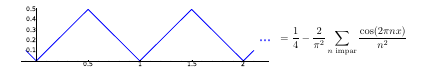
\includegraphics[width=\linewidth]{img/ejemplo_decaimiento.png}
\end{center}

los coeficientes decaen como $n^{-2}$, es decir

\[ \text{ error } \leq \sum_{n \geq N} \frac{1}{n^2}  ≈ N^{-1} \]

Sin embargo en el caso de la sierra

\begin{minipage}{0.5\textwidth}
\begin{center}
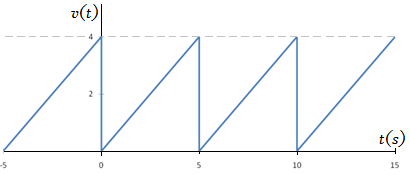
\includegraphics[width=\textwidth]{img/sierra.png}
\end{center}
\end{minipage}
\begin{minipage}{0.5\textwidth}
\[ = \frac{1}{2} - \frac{1}{\pi} \sum^{\infty}_{n = 1} \frac{\sin(2 \pi n x)}{n}\]
\end{minipage}


los coeficientes decaen como $n^{-1}$, es decir:

\[ \text{error } \leq\sum_{n > N} \frac{1}{n} \text{ ni siquiera converge}\]

\obs La regularidad influye en la rapidez de convergencia de la serie de Fourier.


%¿Porqué ocurre que la función que da el diente de sierra es? : $\frac{1}{2} - \frac{1}{\pi} \sum_{n=1}^{\infty} \frac{\sin(2\pi nx)}{n}$

%Esta suma se puede probar que converge (pero la demostración no es fácil en absoluto) pero, excepto para $x = \frac{k}{2}$, se puede probar que la convergencia no es absoluta.

\subsection{Convergencia lenta:}
El problema de la convergencia lenta resulta crítico para las aplicaciones porque nos obliga a almacenar muchos coeficientes de Fourier para obtener la precisión deseada.

\begin{example}
	Si tengo una función $\appl{f}{\ent_N}{\mathbb{C}}$
	$$f(n) = \frac{1}{N}\sum_{m \in \ent_N}\widehat{f}(m)e\left(\frac{mn}{N}\right)$$

	Si tenemos N grande y coeficientes parecidos $\implies$ es difícil decidir cuáles omitir.
\end{example}

\begin{example}
	Supongamos ahora que tenemos una función 1-periódica $\appl{f}{\Pi}{\mathbb{C}}$ tal que $f \in C^{\infty}(\mathbb{R})$.

	Para $n \neq 0$

	$$\widehat{f}(n) = \int_{0}^{1} f(x) e(-nx) dx$$

	Llamamos $\begin{cases}
	u = f(x)\\
	dv = e(-nx) dx
	\end{cases}$

	Entonces:
	$$\widehat{f}(n) = f(x) \left.\frac{e(-nx)}{-2\pi in}\right|_{0}^1 + \frac{1}{2\pi i n} \int_{0}^1 f'(x) e(-nx) dx$$

	Al ser $f(x) \left.\frac{e(-nx)}{-2\pi in}\right|_{0}^1 =0$, como f es periódica, si seguimos iterando hasta k veces llegamos a :

	$$\widehat{f}(n) = \frac{1}{(2\pi i n)^k} \int_{0}^1 f^{(k)}(x) e(-nx) dx$$

	y como $|f^{(k)}| \leq cte$ en [0,1] $\implies |\widehat{f}(n)| \leq \frac{cte}{|n|^k}$
\end{example}

	Con menos regularidad, si $f^{(k)}$ existe excepto en un número finito de puntos (de [0,1]) y está acotada, daría el mismo resultado.

	Vamos a ver esto para $k=2$:

\begin{example}
	$$k=2 \implies |\widehat{f}(n)| \leq cte \implies \sum_{n= -\infty}^{\infty} e(nx)$$
	Converge absolutamente.


\begin{center}
	\centering
	\inputtikz{fourier/audioRepeticionNoContinua}
\end{center}

	La extensión 1-periódica de una función, típicamente no es nisiquiera continua. $\implies$ típicamente no se puede tomar $k=2$ $\implies$ malo para las aplicaciones.

\end{example}

	En estos casos se usa el siguiente truco. En lugar de la extensión periódica primero se refleja la función (la señal) por el eje Y y después se extiende de forma 2-periódica

	Como el reflejo y la señal original coinciden en el final de una y el principio de la otra esta extensión si sería continua


	\begin{center}
		\centering
		\inputtikz{fourier/audio_simetria_simple}
	\end{center}


	Para poder trabajar con esto debemos ver las ecuaciones de Fourier para las funciones 2-periódicas. En este caso

	$$f(x) = \sum_{n=-\infty}^{\infty} \widehat{f}(n)e(n\frac{x}{2}) \text{ siendo }\widehat{f}(n) = \frac{1}{2} \int_{0}^{2} f(x) e(-nx)$$

	Podemos ver que los coeficientes del desarrollo de Fourier para funciones 2-periódicas son reales, siempre y cuando la fucnión $f$ sea real.

	$$\widehat{f}(n) = \frac{1}{2} \int_{-1}^{1} f(x) e(-n\frac{x}{2}) dx = \frac{1}{2} \int_{-1}^{1} f(x)\cos(2\pi n \frac{x}{2})dx \in \mathbb{R}$$

	Esto se debe a que $e(-n\frac{x}{2}) = \cos(2\pi n \frac{x}{2}) + i \sin(2\pi n \frac{x}{2})$ y además f es par y $\sin$ es impar.

	¿Cómo adaptar esto al caso discreto $f: \ent_N \rightarrow \mathbb{C}$?

	\begin{center}
		\centering
		\inputtikz{fourier/extension_2_periodica}
	\end{center}

	Haciendo las cuentas pertinentes se obtiene un análisis de Fourirer discreto en el que podemos usar $e((m + \frac{1}{2}) \frac{n}{2N})$ en vez de $e(\frac{mn}{N})$ y tomando partes reales se puede escribir todo en términos de $\cos(\frac{\pi n}{N}(m+ \frac{1}{2}))$

	\begin{prop}
		Para $f : \{0,1,2....,N-1\} \rightarrow \mathbb{R}$ se cumple
		$$f(m) = \frac{\widehat{f}^c(0)}{N} + \frac{2}{N} \sum_{n=1}^{N-1} \widehat{f}^c(n) \cos\left(\frac{n\pi}{N}\left(m + \frac{1}{2}\right)\right)$$
		donde
		$$\widehat{f}^c(n)= \sum_{m= 0}^{N-1} f(m) \cos\left(\frac{n\pi}{N}\left(m+ \frac{1}{2}\right)\right)$$
	\end{prop}
	\begin{obs} Y esto es lo que más se utiliza en el tratamiento de señales de sonido, imagen, etc
	\end{obs}

	\begin{proof}
		Lo único que hay que hacer es sustituir la definición de $\hat{f}^c (n)$ y comprobar que se tiene una identidad.

		Vamos a abreviar:

		$$f(n) = \sum\limits^{N-1}_{m=0} f(m) \delta(n - m) \;\;\;\;\; \delta(n) = \begin{cases}
			0 & \mbox{si } n \neq 0 \\
			1 & \mbox{si } n = 0
		\end{cases}$$

		Al ser $f $ una combinación lineal de $\delta{-m}$ basta con probar la fórmula para las funciones $f(n) = \delta(n- m_0)$.

		Si escribimos la propiedad para $f(n) = \delta(n - m_0)$ y usamos $2 \cos{(\alpha)} \cos{(\beta)} = \cos{(\alpha + \beta)} + \cos{(\alpha - \beta)}$, lo que hay que probar es:

		$$ \delta(m - m_0) \qeq \frac{1}{N} + \frac{1}{N} \sum\limits^{N-1}{n = 1} \left[ \cos{\frac{\pi n}{N} (m_0 + m + 1)} + \cos{\frac{\pi n}{N} (m - m_0)}   \right] $$

		$$ \delta(m - m_0) \qeq \frac{1}{N} + \frac{1}{N} \sum\limits^{N-1}{n = 1} \left[ \text{Re} \left( e \left( \frac{n}{2N} (m_0 + m + 1) \right) \right) + \text{Re} \left( e \left( \frac{\pi n}{2N} (m - m_0) \right) \right)   \right] $$

		Duplicaríamos la $n$ si añadimos los negativos o los $2N-1, 2N-2, 2N-3,...$.

		$$ = \frac{1}{2N} \text{Re} \sum\limits^{2N-1}_{n=0} \left( e \left( \frac{n}{2N} (m_0 + m + 1) \right) + e \left( \frac{\pi n}{2N} (m - m_0) \right) \right) $$

		$$ \sum\limits^{M - L}_{k = 0} e \left( \frac{k}{M} l \right) = \begin{cases}
			0 & \mbox{si } l \not\equiv 0 \; (M) \\
			M & \mbox{si } l' \equiv 0 \; (M)
		\end{cases}$$

		$\Rightarrow$ la expresión de arriba es $\delta(m - m_0).$

		(prueba supuestamente sencilla teniendo en cuenta que $m-m_0$ varía entre 0 y $N-1$)

	\end{proof}


\section{Aplicaciones}

	\subsection{Formato JPEG}

		\begin{center}
			\inputtikz{fourier/matriz_imagen}
		\end{center}

		Cada píxel son 3 números (bytes) (RGB) (si tiene transparencia 1 más correspondiente al canal alfa)

		R,G,B $\in$ [0,255] (enteros)

		Como hay combinaciones de R y G que se parecen demasiado para el ojo humano, en la realidad casi siempre se pasa de RGB a Y$\text{C}_{\text{B}}$ $\text{C}_{\text{R}}$ con un ``cambio de base'' = con una transformación lineal.

		\begin{itemize}
			\item Y = luminancia $\rightarrow$ el ojo es muy sensible a ella
			\item $\text{C}_{\text{B}}$ Crominancia $\rightarrow$ el ojo es poco sensible a ella.
			\item $\text{C}_{\text{R}}$ Crominancia $\rightarrow$ el ojo es poco sensible a ella.
		\end{itemize}


		En lo que respecta a $\text{C}_{\text{B}}$ y $\text{C}_{\text{R}}$ de omite píxeles (como considerar una foto escalada).

		Imágenes en tonos de gris $\rightarrow$ cada píxel tiene R=G=B y son igules a Y.Nos restringimos a este caso. El general es igual repetido 3 veces.

		\begin{center}
			\inputtikz{fourier/imagen_en_bloques}
		\end{center}

		La imagen $N \times M$ se divide en bloques $8 \times 8$\footnote{Si la imagen no tiene un número de píxeles múltiplo de 8×8, entonces nos \textit{inventamos} píxeles para que cuadre}. Cada uno de ellos se puede interpretar como una función:

		$f:\{0,1,...7\} \times \{0,1,...7\} \rightarrow \mathbb{R}$ que asigna al píxel $P_{ij}$ del bloque, su color (R,Y,G,B $\in [0,255]$) (solo un número para nuestro caso de tonos de gris).


		\textbf{Idea} Descomponer $f$ por Fourier y suprimir las frecuencias altas excepto si tienen coeficientes (amplitudes) grandes.



		En principio, con 3 de estas funciones $f$ tenemos toda la información de los píxeles del bloque.

		\textbf{Cosa técnica:} Al utilizar $Y C_B C_R$, si cambiamos el tono azul, no se aprecia diferencia. Además, para $C_B C_R$ se suelen despreciar entre la mitad y las $\frac{3}{4}$ partes de los píxeles de la imagen original.


		\subsubsection{Aplicación de la DCT (transformada coseno discreta) en cada variable}

			Sabíamos $f: \{ 0,1,...7 \} \rightarrow \mathbb{R}$

			$$ f(m) = \sum\limits^{7}_{n=0} \alpha_n \cos \left(\frac{\pi n}{8} (m + 1/2) \right) \;\;\;\;\; \alpha_n = \text{cierta fórmula} $$

			Si utilizamos esta fórmula en cada variable de F se tiene el desarrollo de Fourier

			$$ F(k,l) = \sum\limits^{7}_{n = 0} \sum\limits^{7}_{m = 0} a_{nm} \cos \left( \frac{\pi n}{8} (k+1/2)  \right) \cos \left( \frac{\pi n}{8} (l+1/2)  \right) $$


			En principio los $a_{nm}$ son 64 números que determinan $F$ pero más dificiles de almacenar explícitamente (son reales, no enteros)

			\begin{framed}
				\vspace{-1.5em}
				\begin{example}

					Si pensamos que -1 es negro y 1 es blanco, $\Phi_{nm}$ es una imagen 8x8 (en tonos de gris) y que $F$ corresponde también a tonos de gris.

					$F = \sum \sum a_{nm} \Phi_{nm}$ es la descomposición de $F$ como superposición de imágenes básicas.

					(IMAGEN POSTCRIP CHAMIZO)

					$\Phi_{00} = 1 $ La que menos oscila.

					$\Phi_{77} = $ la que más oscila.


					\begin{obs} En la práctica los $a_{nm}$ no se calculan con mucha precisión. En GIMP en opciones avanzadas está el DCT method que permite controlar la precisión, pero no se aprecia ninguna diferencia en la imagen aunque si en el tamaño.
					\end{obs}

				\end{example}
			\end{framed}


		\subsubsection{Cuantificación (cuantización)}

			Queremos conseguir elegir el grado de precisión de conversión de la imagen.

			Si tenemos enteros de 1 byte de dos tipos: A y B. Los A son importantes y los B son la mitad de importantes. Podemos almacenarlos de la forma siguiente:
			\begin{itemize}
				\item A $\rightarrow$ tal como están
				\item B $\rightarrow$ divididos entre dos (redondeando si es necesario)
			\end{itemize}

			$$ a_{n} \xrightarrow{almacenar} a_n : 8 \text{ bits } \xrightarrow{recuperar} a_n $$

			$$ b_n \xrightarrow{almacenar} \left[ \frac{b_{n} + 1}{2} \right] : 7 \text{bits} \xrightarrow{recuperar} 2 \left[ \frac{b_n+1}{2} \right] \approx b_n \text{con imprecisión de 1} $$


			En general:

			$$ b \rightarrow \left[ \frac{b}{n} + \frac{1}{2} \right] \rightarrow n * \text{valor almacenado} = b \text{ con imprecisión comparable a n} $$

			$\left[ \frac{b}{n} + \frac{1}{2} \right]$ es el entero más cercano a $\frac{b}{n}$

			valor almacenado solo toma valores múltiplos de n

			n mayor $\rightarrow$ menos números posibles que almacenar pero menos precisión


			Con experimentos se estudia la sensibilidad media del ojo humano a cada $\Phi_{nm}$. Dependiendo de ello se crea una matriz de cuantificación. La usada generalmente para el canal Y es:


			$$ C = \left(\begin{matrix}
			16 & 11 & & & \\
			12 \\
			& & & 120 & 101 \\
			& & & 103 & 99 \\
			\end{matrix}\right)
			$$

			Donde $C_{ij} = $ sensibilidad a distinguir $\phi_{ij}$
			\begin{itemize}
				\item $C_{ij}$ pequeño $\rightarrow$ más sensibilidad
				\item $C_{ij}$ grande $\rightarrow$ menos sensibilidad
			\end{itemize}

			Cada $C_{ij}$ se usa para llevar a cabo una cuantificación de $a_{ij}$.

			Hay otra matriz para $C_B$ y $C_R$

			\begin{framed}
				En resumen

				$$ F \xrightarrow{DCT} \{ a_{nm} \}^{7}_{n,m = 0} \xrightarrow{cuantificación} \left\{ \left[ \frac{a_{nm}}{C_{nm}} + \frac{1}{2} \right] \right\}^{7}_{n,m = 0} $$

				Donde $\left\{ \left[ \frac{a_{nm}}{C_{nm}} + \frac{1}{2} \right] \right\}^{7}_{n,m = 0}$ es el entero más cercano a $\frac{a_{nm}}{C_{nm}}$
			\end{framed}


			Entonces vemos que partiendo de F, tenemos información de 64 bytes, y al hacer $\{\lambda_{nm}\}^7_{m.n=0}$ también tenemos 64 bytes.

			¿Qué hemos ganado?

			Muchos de los $\lambda_{nm}$ son nulos.
			La mayor parte de los bloques $8x8$ no presentan variaciones abruptas. $\implies$ los coeficientes de Fourier decaen rápido.

			Entonces los $a_{nm}$ suelen ser pequeños excepto si $0 \leq n$ , $m \leq 1$ o al menos si $0 \leq n$ , $m \leq$ cte pequeña

			$\implies$ Los $\lambda_{nm}$ correspondientes son nulos típicamente.

			La colección de los $\lambda_{nm}$ corresondientes a todos los bloques está formada mayoritariamente por ceros.

			\begin{example}
				Una imagen con un  $90\%$ de ceros se reconoce bien. Se nota que no es de calidad pero bueno.
			\end{example}

			Además, por la cuantificación, típicamente los números pequeños están muy repetidos.

		\subsubsection{Compresión}
			Se aplica \textbf{compresión Huffman} (típicamente) a los $\lambda_{nm}$

			La compresión normalmente consiste en, en vez de guardar en un fichero todos los ceros que hay, cada vez que vea un cero lo guardo y seguidamente guardo el número de veces que se repite , hasta que aparezca un 1. Se gana mucho ya que normalmente solo uno de cada 100 números es un 1.

			La \textbf{compresión de Huffman} no es exactaente esto, lo que hace es analizar el fichero , ver qué simbolos se repiten más y les asigna códigos para comprimirlos, de manera que optimiza la compresión.

			Esto se contará mejor en el próximo capítulo.


			El resultado de todo esto es el fichero \texttt{.jpg}\\\\


			\textbf{¿Cómo descodificar un  fichero \texttt{.jpg}?}

			Se descomprime el fichero. En la cabecera está toda la información general ( p.ej: la matriz de cuantificación)

			Multiplica los $\lambda_{nm}$ por los $C_{nm}$

			$$\lambda_{nm} \rightarrow C_{nm}\cdot \lambda_{nm} \approx a_{nm} \rightarrow F = \sum \sum a_{nm} \cdot \Phi_{nm}$$

			que reconstruye cada bloque.

	\subsection{Aproximación de funciones}

		Buscamos una manera de enseñarle a un ordenador o una calculadora cómo calcular funciones ``complicadas'' ( seno, coseno, exponencial...).


		Tomamos $ +,-, \cdot \text{ y } \div$ como operaciones básicas. $\implies$ Evaluar polinomios es fácil.

		¿Es posible aproximar muy bien funciones complicadas por polinomios con pocas operaciones?


		Para esto Taylor no sirve ya que sirve muy bien alrededor de un punto, pero cuando nos salimos de ahi no funciona bien.




		La situación típica es que sólo necesitemos aproximar una función en un intervalo.
		$f(x) = \sin x \quad I= [0, \pi/2] \quad x > \pi/2 \rightarrow x - 2\pi k \in [0, 2\pi]$ y después usar $\sin (\pi - x) = \sin (x)$.

		$f(x) = \log x \quad I= [1, 2] \quad x > 2 \rightarrow \log (x) = \log(x / 2^n) + n \log 2$.

		La mayoría de operaciones realizadas por este método (dividir entre 2, elevar 2 a n, ...) son practicamente inmediatas usando la representación binaria del número.



		Con una transformación lineal podemos suponer que el intervalo es $I = [-1,1]$. Queremos aproximar $f: I = [-1,1] \rightarrow \mathbb{R}$ y para ello, desarrollamos por Fourier (pensándolo teoricamente ya que hay infinitos coeficientes), $g(x) = f(\cos(2 \pi x))$.

		$$f(\cos (2 \pi x)) = g(x) = \sum\limits^{\infty}_{n = -\infty} \hat{f}(n) e(nx) = a_0 + 2 \sum\limits^{\infty}_{n=1} a_n \cos(2 \pi nx)$$

		\begin{obs}
			$g$ par $\Rightarrow \hat{f}$ reales. Por lo tanto quitamos la parte imaginaria.
		\end{obs}

		Escribimos el resultado superior tan ``raro'' para poder escribir una formula para todos los coeficientes:

		$$ a_n = \int^{1}_0 g(x) \cos (1 \pi n x) dx $$

		Tomando en el desarrollo $x \rightarrow \frac{1}{2 \pi} \text{arccos} x$ :

		\frame{$f(x) = a_0 + 2 \sum\limits^{\infty}_{n = 1} a_n T_n (x)$} donde

		\begin{op}{Polinomios de Chebyshev}
			T_n (x) = \cos (n \text{arccos} x)
		\end{op}

		\begin{obs}
			$T_n (x)$ es un polinomio para $n \geq 0$, $x \in [-1,1]$.
		\end{obs}

		\begin{example}
			$T_0 (x) = 1$

			$T_1 (x) = \cos (\text{arccos} x) = x$

			$T_2 (x) = \cos (2 \text{arccos} x) = 2 (\cos (\text{arccos} x))^2 - 1 = 2x^2 - 1$

			$T_3 (x) = 4x^3 - 3x$
		\end{example}


		Usando las fórmulas de $\cos ( \alpha \pm \beta)$ se puede deducir que:

		$$T_{n+1} (x) = 2 x T_n (x) - T_{n-1} (x) \quad n \geq 1$$

		Como $T_0$ y $T_1$ son polinomios $\Rightarrow$ Todos los $T_n$ son polinomios.

		\begin{obs}
			Por lo tanto si se busca $T_n (x_0)$ basta calcular $T_0 (x_0)$ y $T_1 (x_0)$ y usar esta fórmula recurrente.
		\end{obs}

		$$
		\begin{aligned}
		f \text{ muy regular} & \Rightarrow g(x) = f(\cos (2 \pi x))\text{ es muy regular y es 1-periódica.} \\
		& \Rightarrow \text{sus coeficientes de Fourier tienden rápido a cero} \\
		& \Rightarrow a_n \rightarrow 0 \text{ muy rápido} \\
		& \Rightarrow f(x) \equiv a_0 + 2 \sum\limits^{N}_{n=1} a_n T_n (x) \text{ es buena aproximación.} \\
		\end{aligned}
		$$

		\begin{obs}
			Los coeficientes $a_n$ pueden ser precalculados y almacenados en memoria.

			$$ a_n = \int^{1}_{0} g(x) \cos (2 \pi n x) dx = - \int^{1}_{0} g'(x) \frac{\sin (2 \pi n x)}{2 \pi n} dx $$

			También se puded determinar el N de antemano dependiendo de la precisión exigida.
		\end{obs}


		\begin{example}{¿Cómo aproximar $\sin (x)$?}

			$$f(x) = \sin(\frac{\pi}{2} x) $$

			Aproximando $f$ en $[-1,1]$ deducimos $\sin$ en $\mathbb{R}$. Y por la simetría impar de $f$ se puede ver que $a_{2k} = 0$.

			$$\sin (\frac{\pi}{2} x) \equiv 0.5668...$$

			$x = T_1 (x) - 0.068 ...$

			$4x^3 - 3x = T_3 (x) + 0.0022 ...$

			$16x^5 - 20x^3 + 5x = T_5(x) ... $

			error absoluto máximo $< 7 * 10^{-5}$

			Con 8 coeficientes no nulos ya se obtiene el error necesario para la doble precisión ($ < 10^{-16}$ por el epsilon máquina).


		\end{example}

\subsubsection{Tomografía}
\begin{itemize}
	\item \textbf{TAC} (Tomografía axial computarizada)
	\item \textbf{RMN} (resonancia magnética nuclear)
\end{itemize}

	Ambas técnicas tienen que ver con el análisis de Fourier

	\textbf{RMN} Resulta que las partículas subatómicas tienen un momento magnético, se comportan como un imán.

	Esos imanes pueden estar cambiando de posición, pero no se puede haer a cualquier velocidad.
	Se ve que con cierta velocidad logras que esto entre en resonancia. \textbf{Esto no lo vamos a ver este curso.}

	\textbf{TAC}

	¿Se puede reconstruir la esctructura de un tejido a través de radiografías?

	La respuesta es SI, ahora vamos a ver cómo.


	Cuando hacemos una radiografía pasamos rayos x por una muestra vemos que al llegar al otro lado los rayos llegan más atenuados si han pasado por zonas de más densidad.

	La "radiografía unidimensional" que se obtiene en el detector (donde llegan los rayos), depende de la integral de la densidad de la muestra a lo largo de la linea.

	En la práctica el emisor y el receptor se van girando y se obtienen los datos correspondientes a todas las radiografías.

	$$r_{\theta , t} \equiv x \cos\theta + y\sin\theta = t$$

	\begin{center}
		\centering
		\inputtikz{fourier/tac}
	\end{center}

	siendo $\theta$ el ángulo con el eje OX y $t$ la distancia de la recta a O (origen).

	 \begin{center}
		\centering
		\inputtikz{fourier/tac_datos}
	\end{center}


En definitiva si $\rho$ = densidad de la muestra. Los datos obtenidos por una máquina de TAC son valores de:

$$P_{\theta} (t) = \int_{r_{\theta , t}} \rho$$

Al final si el patrón que obtengo es más claro, habré pasado por una parte de la muestra con menos densidad, y cuando más oscuro, más densidad.

La pregunta matemática es si a través de los valores de $P_{\theta}(t)$ cuando $\theta$ y $t$ varían es posible recuperar $\rho$

La respuesta a esto la dio J.Radón , que demostró que si que era posible. ¿cómo?

Recordemos la fórmula de $r_{\theta,t}$

	$$r_{\theta , t} \equiv x \cos\theta + y\sin\theta + t$$

	$$P_{\theta} (t) = \int_{r_{\theta , t}} \rho $$

	Entonces, haciendo una parametrización de la recta nos queda:
	$$\int \rho = \int \rho (\phi(u)) \cdot |\phi '(u)| du$$
	\begin{itemize}
		\item $x = t\cos\theta - u \sin\theta$
		\item $y = t\sin\theta + u \cos\theta$
	\end{itemize}

	$$P_{\theta} (t) = \int_{r_{\theta , t}} \rho = \int_{-\infty}^{\infty} \rho ( t\cos\theta - u\sin\theta , t\sin\theta + u\cos\theta) du$$

	Porqué no hemos multiplicado por la norma de la derivada? porque da 1.

	Consideramos la transformada de Fourier de t $\rightarrow P_{\theta}(t)$

	$$\widehat{P_{\theta}}(\xi) = \int_{-\infty}^{\infty} \int_{-\infty}^{\infty} \rho ( t\cos\theta - u\sin\theta , t\sin\theta + u\cos\theta) du\text{  }e(-t\xi) dt $$

	Haciendo un cambio de variable en dos variables $(u,t) \rightarrow (x,y)$ e que corresponde a la paramerización anterior.

	$$\left(\begin{matrix}
		x\\
		y
	\end{matrix} \right) = \left( \begin{matrix}
	\cos & -\sin\\
	\sin & \cos
	\end{matrix}\right)\left(\begin{matrix}
	t\\
	u
	\end{matrix}\right) \longleftrightarrow \left(\begin{matrix}
	t\\
	u
	\end{matrix} \right) = \left( \begin{matrix}
	\cos & \sin\\
	-\sin & \cos
	\end{matrix}\right)\left(\begin{matrix}
	x\\
	y
	\end{matrix}\right)$$

	$$\widehat{P_{\theta}}(\xi) = \int\int_{\real^2} \rho(x,y) e(-\xi(x\cos + y\sin)) dxdy$$

	\obs Como sabemos que $\widehat{f}(\xi) = \int_{-\infty}^{\infty} f(x) e(-x\xi)dx$ Para $F : \real^2 \rightarrow \mathbb{C}$ la definición es similar tomando transformadas en cada variable.

	$$\widehat{F}(\xi , n) = \int \int_{\real^2} f(x,y) e (-x\xi -yn) dxdy$$

	Para intentar no mezclar las variables vamos a usar $r$ en la siguiente fórmula en vez de $\xi$:

	$$\hat{P_{\theta}} (r) = \hat{\rho} (r \cos \theta, r \sin \theta)$$

	$$ \text{Esto implica que } \rho (x,y) = \int_{\real^2} \hat{\rho}(\xi, n) e(x \xi + yn) d\xi dn $$

	Cambiando a polares con $\xi = r \cos \theta$ y $n = r \sin \theta$:

	$$ \rho (x,y) = \int^{2\pi}_{0} \int^{\infty}_{0} r \hat{P}_{\theta} (r) e (x r \cos \theta + y r \sen \theta) dr d\theta $$

	Este sistema se ha tardado mucho en aplicar porque puede funcionar bien en objetos cuya densidad decae suavemente, pero el cuerpo humano no es así, y aunque el cálculo no sea muy complicado, hace falta ordenadores para relizarlo.



%% Cllase práctica


\subsection{Experimentos con imágenes y su transformación de Fourier}

	\subsubsection{Máscaras sobre los coeficientes de Fourier}

		Una vez tenemos los bloques de 8x8, aplicamos máscaras a los coeficientes que se vana a guardar. Esta máscara es una matriz en la que un 1 indica que se debe guardar ese índice, y un 0 indica que no se debe guardar.

		Como cabe esperar, con una matriz llena de unos no hay ninguna diferencia entre la imagen transformada y la imagen original, sin importar que imagen utilicemos para calcularlo.

		Si probamos, por ejemplo, con una matriz llena de ceros excepto un uno en una esquina (la superior izquierda en el ejemplo) lo que ocurre es que para cada bloque de 8 por 8 solo tenemos un coeficiente. Dejando este lo que pasa es que cada bloque de 8x8 tendrá solo un color.

		Seguimos probando, esta vez con una matriz con solo unos excepto por la última fila y la última columna, que tienen 0. Esto descarta 64 - 49 coeficientes. La imagen final no presenta cambios a simple vista, pero podemos observar, sobre todo en dibujos, que en zonas de cambio abrupto hay pequeñas muestras de oscilaciones.


		Podemos seguir quitando las últimas columnas y filas, y con una más todavía seguimos distinguiendo la imagen bastante bien solo que la pérdida de calidad es visible al hacer zoom y comprobar el resultado.

		¿Pero que pasa si quitamos el primer coeficiente? Este es el que indica el promedio de color en ese bloque de la imagen. Si creamos una máscara que descarte solo este coeficiente podremos observar como el promedio no se tiene en cuenta en la imagen transformada. A efectos prácticos, las zonas en las que los colores sean mayoritariamente constantes se verán negras (color 0) ya que el único coeficiente usado sería el promedio (pero lo descartamos) .;ientras que seremos capaces de observar las partes que varían en la imagen van a tener colores distintos del negro, y las vamos a poder ver. Si invertimos la imagen, para que las zonas uniformes se vean blancas la imagen quedará como un dibujo ya que solo se van a ser oscuras las zonas de cambio (en general, los bordes).

	\subsubsection{Comparación entre Fourier y Taylor}

		Con un simple programa de matlab podemos comparar la diferencia entre la aproximación de Taylor a la función $\tan(x \pi/4)$ y la de Fourier. Entre 0 y 1 la aproximación de Fourier y la función real sonindistinguiibles. Calculando el error vemos que es del orden de $10^{-3}$. En cambio, Taylor muestra una gran aproximación en el punto 0, pero se puede apreciar que se empieza a separar notablemente de la función según se acerca a 1 o -1.

		Si probamos con una función más plana vemos como Taylor aproxima mejor que Fourier en el punto pero se separa enseguida, mientras que la de Fourier se mantiene cerca de la función.

	\subsubsection{Más máscaras: Filtros de dibujo}

		Si extendemos ahora el concepto de máscara anterior podemos poner pesos a cada coeficiente si multipliamos cada uno de ellos por su correspondiente peso en la matriz. Y entonces empezamos a buscar matrices que nos consigan un efecto de detección de bordes.

		Vamos a repasar un concepto de la convolución en imágenes. Vamos a verlo primero en 1 variable para entenderlo mejor.

		Si tenemos una $f(x)$ de la que tomamos unos valores (discretizamos) tenemos una sucesión $\{f(n)\}$. Definimos una función: $g(n) = f(n-1) - 2 f(n) + f(n+1)$

		Este filtro  puede parecer absurdo, ya que en una función continua, los valores van a ser muy parecidos, pero la utilidad de este filtro es encontrar discontinuidades, porque los valores son más distantes. ¿Pero y esto no se ve a simple vista? Pues cuando tenemos una imagen, esta es la manera de encontrar los bordes rápidamente (no sólo los bordes de la imagen entera, sino bordes de elementos de la imagen).
		Podríamos hacer el filtro más complicado, en plan $g(n) = f(n-2)+ 2f(n-1) - 5 f(n) + f(n+1) + f(n+1)$, es decir, utilizamos la lista $[1,2,-5,1,1]$ que nos da el filtro aplicado. (En el caso anterior tendríamos $[1,-2,1]$).

		Pero lo útil de esto es en imágenes, como ya hemos dicho, en donde el filtro se representa como una lista en 2 dimensiones, es decir, como una matriz.

		Para entender mejor cómo funciona esto, podemos pensar qué ocurriría con un filtro representado con \[ \begin{pmatrix} 1&1&1\\1&1&1\\1&1&1 \end{pmatrix} \]

		Lo que pasaría es que se desenfoca. Cada píxel toma información de sus adyacentes, lo que provoca desenfoque. Para probarlo, en GIMP  podemos aplicar un filtro de convolución y ver cómo ocurre. No solo con GIMP podemos hacer esto (de una manera "transparente" en el sentido de no entender nada), sino que podríamos hacer un código de Matlab para probarlo. Chamizo ha colgado en la Web unos programas para hacer filtros de convolución.

		¿Qué pasaría en una matriz que fuera nula entera, menos en una línea que fueran todo unos?  Esto crea un \emph{filtro de movimiento}, ya que sólo se "desenfoca" horizontalmente.


		Otro filtro interesante es:

		\[ \begin{pmatrix}
			0 & 0 & 1 & 1 & 0 & 0\\
			0 & 0 & 1 & 1 & 0 & 0\\
			1 & 1 & -4 & -4  & 1 & 1\\
			1 & 1 & -4 & -4  & 1 & 1\\
			0 & 0 & 1 & 1 & 0 & 0\\
			0 & 0 & 1 & 1 & 0 & 0
			\end{pmatrix}\]

		¿Esto que hace? Pues este es el secreto del filtro "Dibujo hecho a lápiz". Aplicando este filtro e invirtiendo, una foto se convierte en un dibujo. Si alguien se anima a completarlo con unas fotos que lo enseñen pues se verá mejor.


	\subsubsection{Transformada de Radón}

		Cuando realizamos la transformada de radón con suficientes muetras (por ejemplo, 180 muestras para media circunferencia) observamos nu resultado muy bueno, con unos bordes más suevizados si eso.

		En cambio, podemos ver que este método es muy sensible a la discretización ya que si tomamos solo 18 muestras a lo largo de media circunferencia, tras aplicar la transformación de Radón y su inversa podemos comprobar como aparecen unas trazas extrañas y ruido por la iamgen, aunque todavía se pueden apreciar las zonas de distinta densidad.








